%!TEX root = slide.tex

\section{Métodos de Passagem de Parâmetros}
\begin{frame}[fragile]{Métodos de Passagem de Parâmetros}
	\begin{itemize}
	  \item Acesso a dados
	  \item Apresentar e recuperar valores
	  \item Parâmetros formais e parâmetros reais
	\end{itemize}
	
	Exemplo de parâmetros reais e parâmetros formais em C++
	\begin{lstlisting}[language=c++]
	void soma(int a, int b) {
	    cout << "Soma = " << a+b; 
	}
	int main() {
	    int x = 2;
	    int y = 5;
	    soma(x, y);
	    return 0;
	}
	\end{lstlisting}	
\end{frame}

\begin{frame}[fragile]{Modelos semânticos de passagem de parâmetros}
	\begin{block}{modo entrada (in mode)}
		Os parâmetros formais recebem dados do parâmetro real.
	\end{block}

	\begin{block}{modo saída (out mode)}
		Os parâmetros formais transmititem dados para o parâmetro real.
	\end{block}

	\begin{block}{modo entrada/saída (inout mode)}
		Podem fazer ambos.
	\end{block}
\end{frame}

\begin{frame}[fragile]{Passagem por valor}
	\begin{itemize}
	  \item Implementação para parâmetros em modo entrada 
	  \item O valor do parâmetro real é utilizado para inicializar o parâmetro formal que atua como uma variável local no subprograma. 
	  \item A transferência dos dados pode ser feita por cópia dos valores ou pela transmissão de um caminho de acesso (ponteiro ou referência) para o valor do parâmetro real. 
	\end{itemize}
\end{frame}

\begin{frame}[fragile]{Passagem por valor}
	\begin{itemize}
	  \item O método de passagem por valor é rápida na vinculação e no tempo de acesso.
	  \item Caminho de acesso: Proteção de célula contra escrita.
	  \item Cópia: espaço adicional para armazenamento e as operações de transferência podem ser custosas se o parâmetro for grande.
	\end{itemize}
\end{frame}

\begin{frame}[fragile]{Passagem por resultado}
	\begin{itemize}
	  \item Implementação para parâmetros em modo saída
	  \item Nenhum valor é transmitido na chamada do subprograma.
	  \item Antes que o controle retorne para o chamador o valor do parâmetro formal é copiado para o parâmetro real.
	  \item Dificuldade esta de garantir que o valor inicial do parâmetro real não seja utilizado no subprograma chamado.
	\end{itemize}
\end{frame}

\begin{frame}[fragile]{Passagem por resultado}
	\begin{itemize}
	  \item Colisão de parâmetros reais: Qual será o valor retornado para a?
	\end{itemize}
	Exemplo em C\#
	\begin{lstlisting}[language=csh]
	void atribuicao(out int x, out int y) {
	    x = 29;
	    y = 15;
	}
	...
	f.atribuicao(out a, out a);
	\end{lstlisting}
\end{frame}

\begin{frame}[fragile]{Passagem por resultado}
	\begin{itemize}
	  \item Tempo para avaliar os endereços dos parâmetros reais.
	  \item Chamada list[21] ou no retorno list[5]?
	\end{itemize}
	Exemplo em C\#
	\begin{lstlisting}[language=csh]
	void subprograma(out int x, int index) {
	    x = 23;
	    index = 5;
	}
	...
	sub = 21;
	f.subprograma(list[sub], sub);
	\end{lstlisting}
\end{frame}

\begin{frame}[fragile]{Passagem por valor-resultado}
	\begin{itemize}
	  \item Implementação para parâmetros em modo entrada-saída.
	  \item Combinação da passagem por valor com a passagem por resultado.
	  \item O valor do parâmetro real é usado para inicializar o parâmetro formal que atua como variável local. 
	  \item No termino do subprograma o valor do parâmetro formal é transmitido de volta para o parâmetro real.
	  \item Partilha dos mesmos problemas da passagem por valor e passagem por resultado.
	\end{itemize}
\end{frame}

\begin{frame}[fragile]{Passagem por referência}
	\begin{itemize}
	  \item Implementação para parâmetros em modo entrada-saída.
	  \item Transmissão de um caminho de acesso.
	  \item Vantagem em relação a passagem por valor-resultado: não é necessário espaço duplicado e nem operações de cópia.
	  \item  Desvantagem: o acesso ao parâmetro formal é mais lento do que a passagem por valor devido ao endereçamento indireto.
	\end{itemize}
\end{frame}

\begin{frame}[fragile]{Passagem por nome}
	\begin{itemize}
	  \item Implementação para parâmetros em modo entrada-saída.
	  \item O parâmetro real é textualmente substituído pelo parâmetro formal em todas as suas ocorrências no subprograma.
	  \item O parâmetro formal é vinculado a valores ou a endereços reais.
	  \item A vinculação real é retardada até o momento que o parâmetro formal seja atribuído ou referenciado.
	  \item Usado em tempo de compilação para parâmetros genéricos de subprogramas genéricos em C++, Java 5.0 e C\# 2005.
	\end{itemize}
\end{frame}

\begin{frame}[fragile]{Pilha em tempo de execução}
	\begin{figure}[ht!]
	 \centering
	 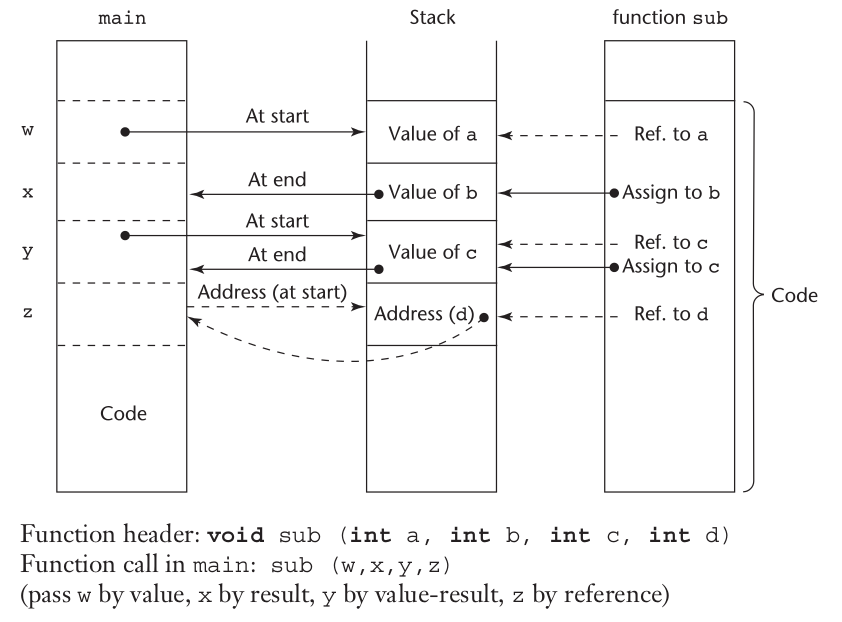
\includegraphics[scale=0.3]{./imgs/run-time-stack.png}
	\label{run-time-stack}
	\end{figure}
\end{frame}

\begin{frame}[fragile]{Métodos de passagem de parâmetros das principais linguagens}
	\begin{itemize}
	  \item O C usa passagem por valor, porém obtêm a semântica da passagem por referência utilizando ponteiros (copiado do ALGOL 68).
	  \item O C++ utiliza também a passagem por valor e garante a passagem por referência com ponteiros.
	  \item O C++ ainda possui um tipo especial de ponteiro chamado tipo de referência que após sua inicialização não pode referenciar outra variável.
	\end{itemize}
	
	\begin{lstlisting}[language=c++]
		void fun(const int &p1, int p2, int &p3) { . . . }
	\end{lstlisting}	
\end{frame}

\begin{frame}[fragile]{Métodos de passagem de parâmetros das principais linguagens}
	\begin{itemize}
	  \item Em Java os parâmetros também são passados por valor, porém como os objetos são apenas acessados por variáveis de referência os parâmetros são passados com a semântica de referência.
	  \item Ada e Fortran 95+ permitem ao programador especificar o modo de cada parâmetro formal (entrada, saída e entrada-saída).
	\end{itemize}
\end{frame}
 

\begin{frame}[fragile]{Métodos de passagem de parâmetros das principais linguagens}
	\begin{itemize}
	  \item O C\# utiliza a passagem por valor como padrão, mas também permite ao programador utilizar passagem por refreferência se o prefixo \textbf{\emph{ref}} for utilizado antes dos dois parâmetros (real e formal).
	  \item Também suporta passagem de parâmetro em modo saída, passado por referência, com o modificador out antes do parâmetro formal.
	\end{itemize}
	\begin{lstlisting}[language=csh]
		void sumer(ref int oldSum, int newOne) { . . . }
		...
		sumer(ref sum, newValue);
	\end{lstlisting}	
\end{frame}
 
\begin{frame}[fragile]{Métodos de passagem de parâmetros das principais linguagens}
	\begin{itemize}
	  \item Em Python e Ruby é utilizado a passagem por atribuição em que todos os valores de dados são objetos.
	  \item Se uma variável referenciada é acrescida de uma unidade então é criado um novo objeto com o valor da variável mais 1 e a variável referencia o novo objeto.
	  \item  No caso de vetor passado como parâmetro se houver uma atribuição ao parâmetro formal que referencia o vetor então não tem efeito no chamador.
	  \item Se houve uma atribuição à um elemento do vetor passado então o correspondente parâmetro real será modificado.
	\end{itemize}
\end{frame}

\begin{frame}[fragile]{Matrizes multidimencionais como parâmetro}
	\begin{itemize}
	  \item Quando uma matriz é passado como parâmetro o compilador deve ser capaz de construir uma função de mapeamento. 
	  \item Uma função de mapeamento simples mapeia valores inteiros (índices de elementos na matriz) para os endereços dos elementos da matriz.
	\end{itemize}
\end{frame}

\begin{frame}[fragile]{Matrizes multidimencionais como parâmetro}
	Exemplo em C
	\begin{lstlisting}[language=c]		
	void procedure(int *mat, int rows, int cols) {
	    ...
	}
	void main() {
	    int mat[2][3];
	    ...
	    procedure(&mat, 2, 3); //ou procedure(mat[0][0], 2, 3);
	    ...
	}
	\end{lstlisting}	
\end{frame}

\begin{frame}[fragile]{Matrizes multidimencionais como parâmetro}
	Exemplo em Ada
	\begin{lstlisting}[language=ada]		
	type Mat_Type is array (Integer range <>, Integer range <>) of Float;

	Mat_1 : Mat_Type(1..5, 1..30);

	function Sumer(Mat : in Mat_Type) return Float is
	    ...
	end Sumer;
	\end{lstlisting}	
\end{frame}